\documentclass[tikz]{standalone}
%\usepackage{pgfplots}
%\pgfplotsset{compat=1.11}
\definecolor{Set1-7-1}{RGB}{228,26,28}
\definecolor{Set1-7-2}{RGB}{55,126,184}
\definecolor{Set1-7-3}{RGB}{77,175,74}
\definecolor{Set1-7-4}{RGB}{152,78,163}
\definecolor{Set1-7-5}{RGB}{255,127,0}
\definecolor{Set1-7-6}{RGB}{255,255,51}
\definecolor{Set1-7-7}{RGB}{166,86,40}
\usepackage{amsmath}
\providecommand{\abs}[1]{\lvert#1\rvert}
\usepackage{mathspec}
\setromanfont[Numbers={Lining,Proportional}]{Minion Pro}
\setmathsfont(Digits,Latin,Greek)[Numbers={Lining,Proportional}]{Minion Pro}
\setmathrm{Minion Pro}

\usepackage{fix-cm}
\begin{document}
\begin{tikzpicture}[level/.style={thick}]

\node[rotate=90] at (0,0) {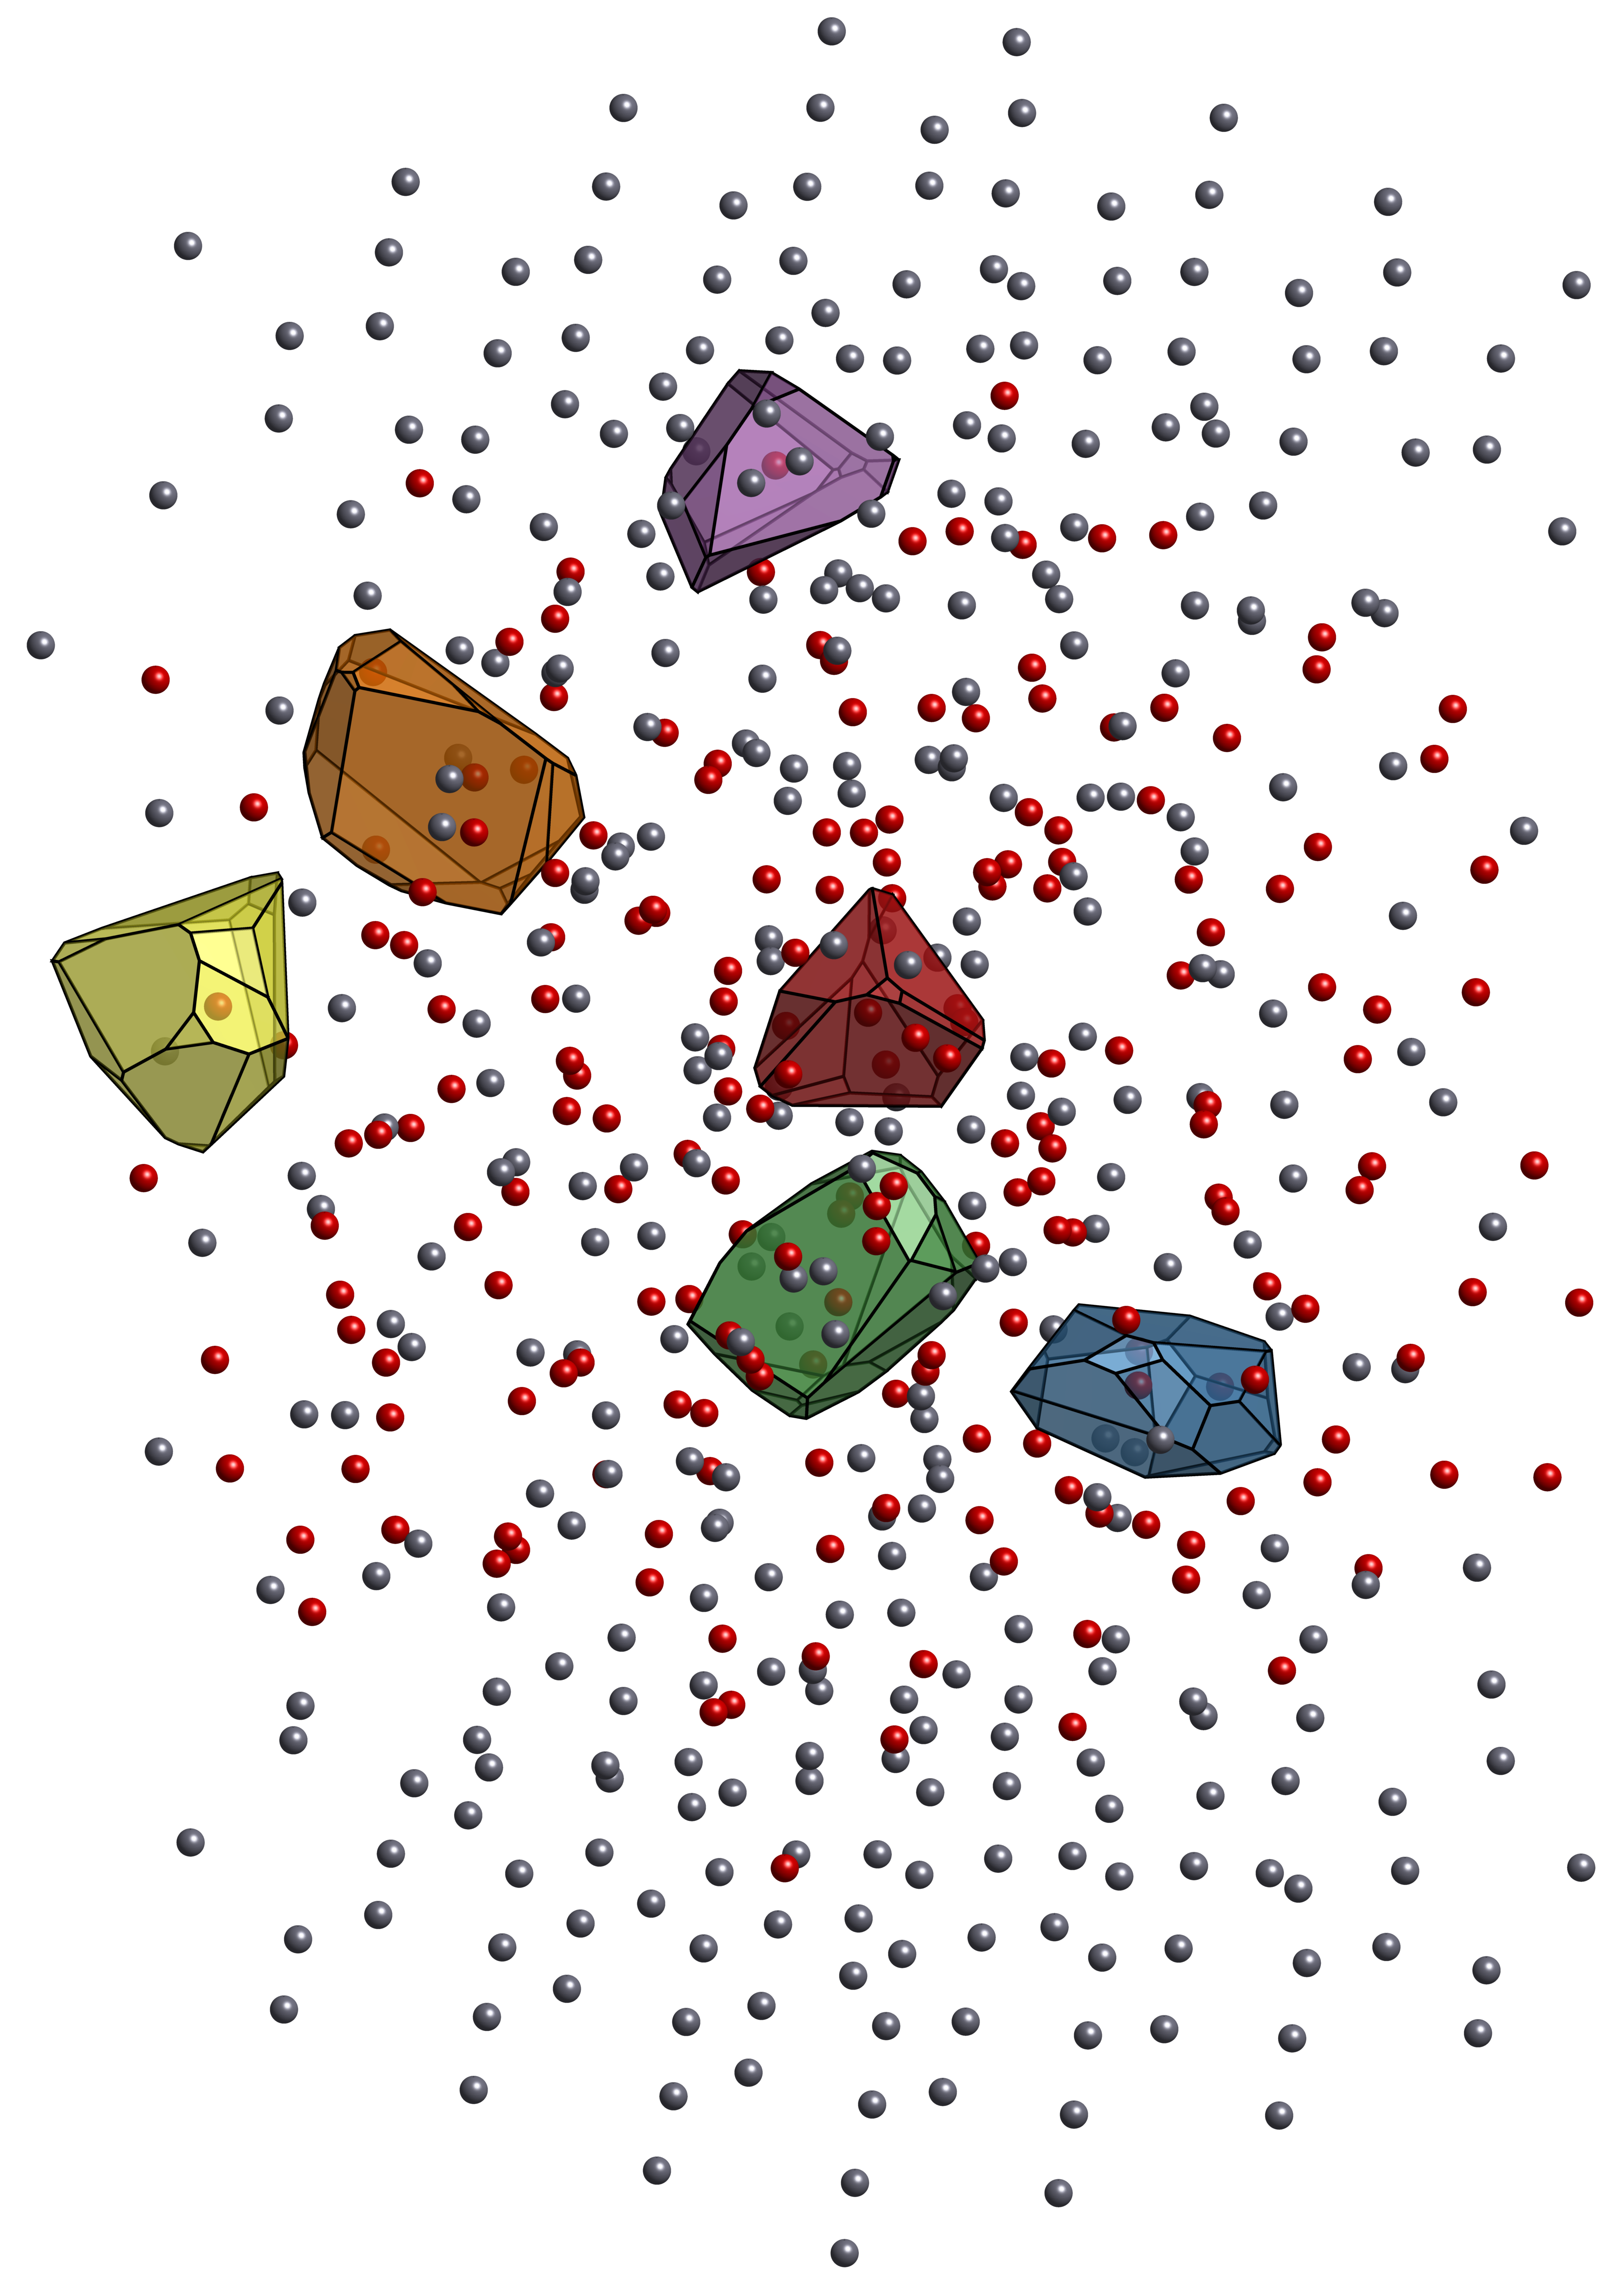
\includegraphics[scale=1]{vors}};

\begin{scope}[yscale=3,xshift=-10cm,yshift=-4.1cm]
    %large3 (purple) proper done
    \filldraw [black,fill=Set1-7-4,fill opacity=0.7] (0,1.25) -- (0.5,1.25) -- (0.5,1.1) -- (0,1.1) --cycle;
    \node at (1.8,1.175) {\Large 6 \includegraphics[width=0.5em]{aluminium}\, 13 \includegraphics[width=0.5em]{oxygen}};
    \node at (4,1.175) {\Large $\xi = 1.72$};

    \draw[level] (3,0) node[above=1.7em, right] {$E_{01} = 22.71$ THz} -- (0,0) node[left] {$E_{0}$};
    \draw[level] (3,0.45) node[above=0.4em, right] {$E_{12} = 5.09$ THz} -- (0,0.45) node[below=0.2em, left] {$E_{1}$};
    \draw[level] (3,0.55) node[above=1.6em, right] {$E_{23} = 17.54$ THz} -- (0,0.55) node[above=0.2em, left] {$E_{2}$};
    \draw[level] (3,0.9) node[above=0.4em, right] {$E_{34} = 5.11$ THz} -- (0,0.9) node[below=0.2em, left] {$E_{3}$};
    \draw[level] (3,1) -- (0,1) node[above=0.2em,left] {$E_{4}$};
    \node at (2.425,-0.2) {\large $\abs{\wp_x} = 0.030, \abs{\wp_y} = 0.020, \abs{\wp_z} = 0.002$ \AA}; %done
\end{scope}

\begin{scope}[yscale=3,xshift=-2cm,yshift=-4.1cm]
    %large4 (orange) proper done
     \filldraw [black,fill=Set1-7-5,fill opacity=0.7] (0,1.25) -- (0.5,1.25) -- (0.5,1.1) -- (0,1.1) --cycle;
    \node at (1.8,1.175) {\Large 9 \includegraphics[width=0.5em]{aluminium}\, 12 \includegraphics[width=0.5em]{oxygen}};
    \node at (4,1.175) {\Large $\xi = 1.50$};

    \draw[level] (3,0) node[above=1.6em, right] {$E_{01} = 22.53$ THz} -- (0,0) node[left] {$E_{0}$};
    \draw[level] (3,0.41) node[above=0.8em, right] {$E_{12} = 11.16$ THz} -- (0,0.41) node[left] {$E_{1}$};
    \draw[level] (3,0.62) node[above=0.8em, right] {$E_{23} = 11.31$ THz} -- (0,0.62) node[left] {$E_{2}$};
    \draw[level] (3,0.83) node[above=0.7em, right] {$E_{34} = 9.37$ THz} -- (0,0.83) node[left] {$E_{3}$};
    \draw[level] (3,1) -- (0,1) node[left] {$E_{4}$};
    \node at (2.425,-0.2) {\large $\abs{\wp_x} = 0.008, \abs{\wp_y} = 0.028, \abs{\wp_z} = 0.021$ \AA}; %done
\end{scope}

\begin{scope}[yscale=3,xshift=6cm,yshift=-4.1cm]
    %large5 (yellow) proper done
    \filldraw [black,fill=Set1-7-6,fill opacity=0.7] (0,1.25) -- (0.5,1.25) -- (0.5,1.1) -- (0,1.1) --cycle;
    \node at (1.8,1.175) {\Large 11 \includegraphics[width=0.5em]{aluminium}\, 13 \includegraphics[width=0.5em]{oxygen}};
    \node at (4,1.175) {\Large $\xi = 1.40$};

    \draw[level] (3,0) node[above=1.6em, right] {$E_{01} = 24.98$ THz} -- (0,0) node[left] {$E_{0}$};
    \draw[level] (3,0.39) node[above=0.9em, right] {$E_{12} = 14.93$ THz} -- (0,0.39) node[left] {$E_{1}$};
    \draw[level] (3,0.62) node[above=0.5em, right] {$E_{23} = 10.29$ THz} -- (0,0.62) node[left] {$E_{2}$};
    \draw[level] (3,0.77) node[above=1.0em, right] {$E_{34} = 14.58$ THz} -- (0,0.77) node[left] {$E_{3}$};
    \draw[level] (3,1) -- (0,1) node[left] {$E_{4}$};
    \node at (2.425,-0.2) {\large $\abs{\wp_x} = 0.013, \abs{\wp_y} = 0.032, \abs{\wp_z} = 0.001$ \AA};
\end{scope}
 
\begin{scope}[yscale=3,xshift=-10cm,yshift=3.5cm]
    %ASYM (RED) Complete
    \filldraw [black,fill=Set1-7-1,fill opacity=0.7] (0,1.25) -- (0.5,1.25) -- (0.5,1.1) -- (0,1.1) --cycle;
    \node at (1.8,1.175) {\Large 5 \includegraphics[width=0.5em]{aluminium}\, 9 \includegraphics[width=0.5em]{oxygen}};
    \node at (4,1.175) {\Large $\xi = 1.44$};

    \draw[level] (3,0) node[above=1.8em, right] {$E_{01} = 11.81$ THz} -- (0,0) node[left] {$E_{0}$};
    \draw[level] (3,0.5) node[above=0.7em, right] {$E_{12} = 4.97$ THz} -- (0,0.5) node[left] {$E_{1}$};
    \draw[level] (3,0.71) node[above=0.1em, right] {$E_{23} = 0.47$ THz} -- (0,0.71) node[below=0.4em, left] {$E_{2}$};
    \draw[level] (3,0.73) node[above=1.1em, right] {$E_{34} = 6.31$ THz} -- (0,0.73) node[above=0.4em, left] {$E_{3}$};
    \draw[level] (3,1) -- (0,1) node[left] {$E_{4}$};
    \node at (2.425,-0.2) {\large $\abs{\wp_x} = 0.035, \abs{\wp_y} = 0.013, \abs{\wp_z} = 0.034$ \AA};
\end{scope}

\begin{scope}[yscale=3,xshift=-2cm,yshift=3.5cm]
    %large2 (green) proper done
    \filldraw [black,fill=Set1-7-3,fill opacity=0.7] (0,1.25) -- (0.5,1.25) -- (0.5,1.1) -- (0,1.1) --cycle;
    \node at (1.8,1.175) {\Large 8 \includegraphics[width=0.5em]{aluminium}\, 11 \includegraphics[width=0.5em]{oxygen}};
    \node at (4,1.175) {\Large $\xi = 1.38$};

    \draw[level] (3,0) node[above=1.4em, right] {$E_{01} = 13.50$ THz} -- (0,0) node[left] {$E_{0}$};
    \draw[level] (3,0.33) node[above=1.3em, right] {$E_{12} = 13.47$ THz} -- (0,0.33) node[left] {$E_{1}$};
    \draw[level] (3,0.67) node[above=0.8em, right] {$E_{23} = 8.66$ THz} -- (0,0.67) node[left] {$E_{2}$};
    \draw[level] (3,0.88) node[above=0.5em, right] {$E_{34} = 4.78$ THz} -- (0,0.88) node[left] {$E_{3}$};
    \draw[level] (3,1) -- (0,1) node[left] {$E_{4}$};
    \node at (2.425,-0.2) {\large $\abs{\wp_x} = 0.026, \abs{\wp_y} = 0.037, \abs{\wp_z} = 0.012$ \AA}; %done
\end{scope}
   

\begin{scope}[yscale=3,xshift=6cm,yshift=3.5cm]
    %large1 (blue) proper done
    \filldraw [black,fill=Set1-7-2,fill opacity=0.7] (0,1.25) -- (0.5,1.25) -- (0.5,1.1) -- (0,1.1) --cycle;
    \node at (1.8,1.175) {\Large 13 \includegraphics[width=0.5em]{aluminium}\, 5 \includegraphics[width=0.5em]{oxygen}};
    \node at (4,1.175) {\Large $\xi = 1.60$};

    \draw[level] (3,0) node[above=1.8em, right] {$E_{01} = 45.30$ THz} -- (0,0) node[left] {$E_{0}$};
    \draw[level] (3,0.48) node[above=1.0em, right] {$E_{12} = 25.46$ THz} -- (0,0.48) node[left] {$E_{1}$};
    \draw[level] (3,0.75) node[above=0.7em, right] {$E_{23} = 19.61$ THz} -- (0,0.75) node[left] {$E_{2}$};
    \draw[level] (3,0.96) node[above=0.2em, right] {$E_{34} = 3.88$ THz} -- (0,0.96) node[below=0.4em, left] {$E_{3}$};
    \draw[level] (3,1) -- (0,1) node[above=0.4em, left] {$E_{4}$};
    \node at (2.425,-0.2) {\large $\abs{\wp_x} = 0.013, \abs{\wp_y} = 0.015, \abs{\wp_z} = 0.017$ \AA};
\end{scope}

\end{tikzpicture}%
\end{document} 